
%(BEGIN_QUESTION)
% Copyright 2012, Tony R. Kuphaldt, released under the Creative Commons Attribution License (v 1.0)
% This means you may do almost anything with this work of mine, so long as you give me proper credit

A {\it programmable logic controller} (PLC) may be used to command a high-voltage circuit breaker to trip in the event of dangerous process conditions, such as the system shown here:

$$\includegraphics[width=15.5cm]{i02113x01.eps}$$

Assume this process system is operating as it should (i.e. no abnormal conditions).  Based on the status LED indicators you see on the input card of the PLC, determine whether each of the process switches is designed to trip on a {\it low} condition or a {\it high} condition.  Then, determine what you would have to do to the circuit to simulate a shutdown condition for each of the process switches (i.e. make the PLC ``think'' it sees an abnormal condition, so that it will act to trip the breaker):

\begin{itemize}
\item{} Temperature switch: trips on {\it low} temperature or {\it high} temperature?  How to simulate trip condition?
\item{} Level switch: trips on {\it low} liquid level or {\it high} liquid level?  How to simulate trip condition?
\item{} Pressure switch: trips on {\it low} fluid pressure or {\it high} fluid pressure?  How to simulate trip condition?
\end{itemize}

\vskip 20pt \vbox{\hrule \hbox{\strut \vrule{} {\bf Suggestions for Socratic discussion} \vrule} \hrule}

\begin{itemize}
\item{} Explain why the LED status indicators are so helpful for system troubleshooting in a PLC-controlled system.
\item{} Identify the purpose of the key switch in this circuit.
\item{} Suppose you were asked to install a manual pushbutton ``Emergency Trip'' switch to trip the circuit breaker.  Where would you connect such a switch in this circuit?
\end{itemize}

\underbar{file i02113}
%(END_QUESTION)





%(BEGIN_ANSWER)

The indicators for channels 3 and 6 are lit on the input card of this PLC.  This tells us channels 3 and 6 are receiving power through their respective process switches, but channel 4 is not.  Since we are told the system is operating as it should (no abnormal conditions), we may assume the opposite state for each input channel will initiate a trip.  Thus:

\begin{itemize}
\item{} Temperature switch (channel 6) is currently closed, and opens with a {\it high} temperature.
\item{} Level switch (channel 4) is currently open, and closes with a {\it low} level.
\item{} Pressure switch (channel 3) is currently closed, and opens with a {\it low} pressure.
\end{itemize}

Since the temperature switch channel is {\it de-energize to trip}, you must open that circuit in order to force the system to trip.

\vskip 10pt

Since the level switch channel is {\it energize to trip}, you must jumper power to PLC input channel 4 in order to force the system to trip.

\vskip 10pt

Since the pressure switch channel is {\it de-energize to trip}, you must open that circuit in order to force the system to trip.




%(END_ANSWER)





%(BEGIN_NOTES)



\vskip 20pt \vbox{\hrule \hbox{\strut \vrule{} {\bf Virtual Trip-testing} \vrule} \hrule}

This question is a good candidate for a ``Virtual Trip-testing'' exercise.  Presenting the diagram to students, you pose an assignment whereby students must figure out how to test some component of this system to check that it will operate as intended to shut down the system in an abnormal (trip) condition, with some realistic limitation (e.g. power cannot be shut off to the load).  Students then propose various methods for executing the test.  Your job is to determine whether or not their proposed tests will achieve the desired result(s).

During and after the exercise, it is good to ask students follow-up questions such as:

\begin{itemize}
\item{} Where might our planned test strategy go wrong?  In other words, what thing(s) might happen to foil our test, either to invalidate the results or to not honor the stated limitation(s)?
\item{} Suppose the limitation were different.  How would this affect our ability to carry out the test?
\item{} Is the last test strategy best one we could execute?
\end{itemize}


%INDEX% Electric power systems: HV circuit breaker controls
%INDEX% Safety, shutdown system: trip testing

%(END_NOTES)


